\chapter{ Literature Review }
\section{Introduction}
The skin is the largest organ in the human body in the region, and is exposed to several external and intrinsic factors that make it prey to a number of diseases. Some are dangerous. Skin diseases have many causes, including those related to biological changes that occur in the human body, such as hormonal disorders, for example. Including what is related to external influences that change the nature of the skin, the most important of which are climatic influences, pollution of the surrounding environment, and so on. However, dietary habits, smoking, lack of sleep as well as psychological stress are all factors that strongly affect the integrity of the skin, and because the freshness of the skin is related to its integrity, it is necessary to pay attention to the health of the skin first. There are many diseases that affect the skin, and they vary according to the diversity of geographical areas. Therefore, in this paper, we presented a complete diagnostic health care system that includes a variety of tools that help patients in the rapid diagnosis and knowledge of the disease and how to prevent it.
Many doctors around the world can identify many skin diseases by examining it directly. But with the advancement of technology, there were a lot of scientists who searched and did research in diagnosing skin diseases, as they presented 
\subsection{In paper\cite{r1}} This was a retrospective study that was an attempt to develop CAD for a more general dermatology that may be of great interest, especially for general practitioners. This was an image-based study using multitasking learning for binary classification.\\\\
All images were diagnosed by AUH-trained dermatologists according to the International Classification of Diseases, 10th Edition (ICD-10).
For the ICD-10 codes included in each disease category, the CTCL diagnosis was histologically verified. 
Best performance was obtained by training the VGG-16 on 16,543 non-standard images. The image data was distributed in the training set (80\%), the validation set (10\%), and the test set (10\%).\\\\

All images were collected from a clinical database of a Danish population attending one dermatology department. Patients classified with ICD-10 codes related to acne, rosacea, psoriasis, eczema, and cutaneous T-cell lymphoma were included.\\\\

Acne was distinguished from rosacea with a sensitivity of 85.42\%, a confidence interval of 72.24-93.93\%, a specificity of 89.53\%, a confidence interval of 83.97-93.68\%. A specificity of 84.09\% CI 80.83–86.99\%, Eczema Psoriasis with a sensitivity of 81.79\% CI 78.51–84.76\% and a specificity of 73.57\% CI 69.76–77.13\%. All results were based on the test set. Notably, this model discriminated between diseases in all three tasks with an accuracy above 77\%, indicating an accuracy of clinical relevance compared to the diagnostic accuracy reported in dermatology in general for primary care physicians (48–77\%).\\\\

Reported performance rates were equal to or higher than those reported for general practitioners with dermatological training, suggesting that computer-aided diagnostic models based on convolutional neural network could potentially be used for the diagnosis of multi-lesional dermatoses.
\subsection{ In paper\cite{r2}}In this study, inflammatory skin disease refers to a cutaneous disorder that involves infiltration of inflammatory cells and severe elevation of inflammatory cytokines.\\\\

 Inflammatory skin diseases affect more than 1/5 of the world's population worldwide.Inflammatory skin diseases include psoriasis (Pso), eczema (Ecz), and atopic dermatitis (AD), dermatologists usually diagnose these diseases by "first impression" and then follow pathological examinations and laboratory tests to confirm the "first impression".However, less experienced dermatologists and young dermatologists are especially prone to errors since Pso, Ecz, and AD are easily misdiagnosed.[Fig. 1]
 \begin{figure}[!ht]
 \centering 
 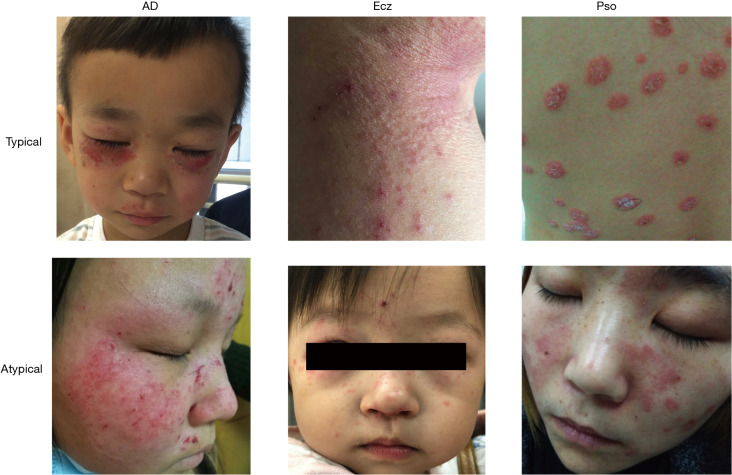
\includegraphics{backmatter/figures/fig.jpg}
 \caption{The images for Pso, AD, and Ecz. Pso, psoriasis; Ecz, eczema; AD, atopic dermatitis.}
 \end{figure}
To solve this problem and help dermatologists, in this study, they developed a comprehensive deep learning model, which is based on clinical skin images, for automated diagnosis of Pso, Ecz, and AD.\\\\

Based on the EfficientNet-b4 CNN algorithm, they developed the Artificial Intelligence Dermatology Diagnostic Assistant (AIDDA) for Healthy Skin (HC), Pso, Ecz and AD.\\\\

The proposed CNN model was trained based on 4,740 clinical images, and performance was evaluated on expert-confirmed clinical images grouped into 3 different diagnostic classifications prescribed by dermatologists (HC, Pso, Ecz \& AD).\\\\
The overall diagnostic accuracy for AIDDA was 95.80\% ± 0.09\%, with a sensitivity of 94.40\% ± 0.12\% and specificity of 97.20\% ± 0.06\%. AIDDA showed an accuracy for Pso of 89.46\%, with a sensitivity of 91.4\% and a specificity of 95.48\%, and an accuracy for AD \& Ecz of 92.57\%, with a sensitivity of 94.56\% and a specificity of 94.41\%.\\\\
Thus, AIDDA is already making an impact in diagnosing inflammatory skin diseases, and highlights how deep learning network tools can help advance clinical practice.
\subsection{In paper\cite{r3}}
Skin diseases affect 1.9 billion people.
Because of the shortage of dermatologists, most cases are examined by general practitioners who have lower diagnostic accuracy.\\\\

They introduced a deep learning system (DLS) to provide a differential diagnosis of dermatology using 16,114 unidentified cases (photographs and clinical data) from a remote dermatology practice serving 17 sites.\\\\
The DLS distinguishes between 26 common skin conditions, representing 80\% of cases seen in primary care, while also providing a secondary predictor covering 419 skin conditions.\\\\
In 963 validation cases, in which a rotating panel of three board-certified dermatologists set the reference standard, DLS was not inferior to six other dermatologists and superior to six primary care physicians (PCPs) and six nurse practitioners (NPs) (top- 1 Accuracy: 0.66 DLS, 0.63 dermatologists, 0.44 PCPs and 0.40 NPs).
\subsection{In paper\cite{r4}}
In this study, training and testing data were obtained from Dermnet NZ, a dermatological information archive launched and maintained by a group of New Zealand dermatologists. The site provides open source images with labels.
To go away, they selected 18 high-level categories (Table 5) each of which included sufficient data, besides including erythema as one of their common symptoms.\\\\

Using a web crawler, they collected a total of 15,851 images.
Among the images obtained through Dermnet, the dermatologists hid my erythema 100 images for use as a base fact.
For segmentation, 60 images were used for training, and 40 images were used for testing.\\\\

For classification, 13473 images were used for training, and 2378 images were used for testing. In addition, the classification test set was split before hash cropping to prevent single image subsections from appearing in both the training and test sets.
They selected 100 images for segmentation in a balanced manner from each category, to minimize any bias that could occur during the classification phase.\\\\
They showed that even without a large data set and high-quality images, it is possible to achieve sufficient resolutions. In addition, they show that current latest CNN models can outperform models generated by previous research, through data preprocessing, self-supervised learning, transfer learning, and proprietary CNN architecture techniques.Moreover, through careful segmentation, they gain knowledge of disease location, which is useful in preprocessing the data used for classification, as it allows the CNN model to focus on the area of interest.\\\\
Our method provides a solution to classify multiple diseases in a single image. With higher quality and greater amount of data, it will be possible to use the latest models to enable the use of CAD in the field of dermatology.

\subsection{In paper\cite{r5}}
In this study, a data sample from the complete data set used to train the system model is presented in[Fig. 2]
\begin{figure}[!ht]
\centering 
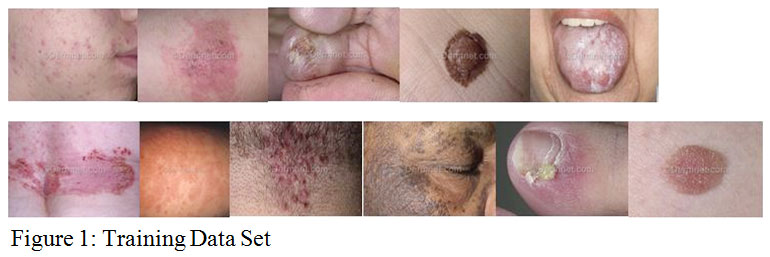
\includegraphics[height= 8cm, width=9cm]{backmatter/figures/fig2.jpg}
\caption{Training Data Set}
\end{figure}.
 The database is divided into; Training set, validation/test set. A training set is adopted to learn to fit the parameters and is specifically applied to vary the variable weights and errors of the system in each training session. The validation/test set adjusts the parameters and is only used to evaluate the effectiveness and efficiency of the system.\\\\
 
 The method uses computer vision related techniques to distinguish between different types of dermal skin abnormalities. They used different types of deep learning algorithms (Inception\_v3, MobileNet, Resnet, xception) for feature extraction and a learning algorithm (preferably Random Forest or Logistic Regression) for training and testing purpose.\\\\
 
 Using modern architecture greatly increases efficiency up to 88 percent. Moreover, by using feature set mapping, combing trained models with Inception V3, MobileNet, Resnet and Xception, a voting-based model will be compiled and thus increase efficiency.\\\\
 
 In order to improve performance and choose the optimal architecture for the application, they have used logistic regression technology. In this method, the division mode is set to 90\% to train the data, and 10\% to validate/test the data. To characterize the efficiency of a classification model (or "classifier") on a set of test data that has true values.\\\\
In this work, a model for predicting skin diseases was made using deep learning algorithms. It has been found that they can achieve a higher accuracy rate and can also predict many more diseases than any other previous models that have been performed before. Also, previous models performed in this field of application were able to report a maximum of six dermatological diseases with a maximum accuracy level of 75\%. By applying a deep learning algorithm, they predicted up to 20 diseases with a higher accuracy level of 88\%.
\subsection{In paper\cite{r6}}
In this article, they report a Deep Learning System (DLS) to identify the 26 most common dermatological conditions in adults referred for teledermatology consultation. As a secondary predictor, DLS also produces predictions for the full cohort of the 419 skin conditions seen in this work. Their DLS offers many improvements over previous work.\\\\
First, rather than individual classification among a small number of conditions, their DLS provides a differential diagnosis across 26 conditions, including different skin conditions, dermatoses, pigmentary conditions, alopecia and lesions, to aid clinical decision-making.\\
Second, rather than relying solely on images, DLS makes use of the 45 types of data available to dermatologists in the remote dermatology service, such as demographic information and medical history.\\
Third, DLS supports a variable number of input images, and the usefulness of using multiple images has been evaluated. Finally, to understand the potential value of DLS, they compared its diagnostic accuracy with that of board-certified physicians with three different levels of training: dermatologists, PCPs and NPs.They used Inception-v4 modules with shared weights before applying an argument set and binding to metadata features.\\\\

The primary output of the DLS classification layer is the relative probability of 27 classes (26 skin conditions plus “others”). The byproduct is the relative probability of a complete set of 419 skin conditions seen in this work.Their DLS has two main components: a variable number of deep convolutional neural network modules for processing a flexible number of input images, and a shallow module for processing metadata such as demographic information and medical history\\\\

To develop and validate their DLS, they applied a chronological breakdown of 36 remote skin cases: the first 80\% (years 2010–2017) to development and the last 20\% (years 2017–2018) to validation.\\\\
The reference standard for each case was determined by the pooled opinions of dermatologists who reviewed the case independently (see Methods). After excluding cases with multiple skin diseases and those that could not be diagnosed, 16,114 (64,837 images) were used for development and 3,756 (14,883 images) for validation (validation set A; smaller subset B used for comparison with clinicians and described in sections related to). In all, 64,878 dermatological reviews were collected for development and 11,268 for validation. , where he found higher accuracy 1 = 0.71 \& higher 1 sensitivity = 0.58 higher accuracy 0.93 \& sensitivity = 0.83\\\\
In the following sections, we will explain the different libraries and tools that we used to create our integrated health system capable of diagnosing skin diseases and determining how to treat them.
\section{Background}
The system we are going to build, DermAI, will depend on artificial intelligence technologies, soft computing techniques and a mobile application to operate. The following subsections provide a brief background information about tools, and techniques needed to build our system including TensorFlow, Numpy, Jinja, Toml, Guzzle, Sanctum, and Programming Languages.
\subsection{Keras}
Keras is an open source software library that provides a Python interface for artificial neural networks. Keras acts as an interface to the TensorFlow library. Keras has supported several backends, including TensorFlow, Microsoft Cognitive Toolkit, Theano, and PlaidML.
\subsection{TensorFlow}
TensorFlow is a free and open-source software library for machine learning and artificial intelligence. It can be used across a range of tasks but has a particular focus on training and inference of deep neural networks.
\subsection{Flask}
Flask is a web framework that provides libraries to build lightweight web applications in python. It is developed by Armin Ronacher who leads an international group of python enthusiasts (POCCO). It is based on WSGI toolkit and jinja2 template engine. Flask is considered as a micro framework.
\subsection{Numpy}
NumPy is a library for the Python programming language, adding support for large, multi-dimensional arrays and matrices, along with a large collection of high-level mathematical functions to operate on these arrays.
\subsection{Jinja}
Jinja is a web template engine for the Python programming language. Jinja is similar to the Django template engine but provides Python-like expressions while ensuring that the templates are evaluated in a sandbox.
\subsection{Toml}
Toml is the specified file format of PEP 518 which contains the build system requirements of Python project.
\subsection{Laravel}
Laravel is an open-source PHP framework, which is robust and easy to understand. It follows a model-view-controller design pattern. Laravel reuses the existing components of different frameworks which helps in creating a web application.
\subsection{Guzzle}
Guzzle is a PHP HTTP client that makes it easy to send HTTP requests and trivial to integrate with web services.
\subsection{Sanctum}
Sanctum is a simple package you may use to issue API tokens to your users without the complication of OAuth. This feature is inspired by GitHub and other applications which issue "personal access tokens". For example, imagine the "account settings" of your application has a screen where a user may generate an API token for their account. You may use Sanctum to generate and manage those tokens. These tokens typically have a very long expiration time (years), but may be manually revoked by the user at anytime.
\subsection{Android}
Android is a mobile operating system based on a modified version of the Linux kernel and other open source software, designed primarily for touchscreen mobile devices such as smartphones and tablets. we used java and kotlen.

\section{Review of Relevant Work }
After studying quite a few research papers in scientific journals, some of which were mentioned above, we came to the conclusion that the use of AI tools is a promising method for diagnosing common diseases and an additional, comparatively easier and cheaper additional asset.\\\\
To help the lack of health care services and personnel, but sometimes the accuracy of an independent model system may not suit all types of diseases, moreover, its accuracy may fluctuate depending on the disease. These problems make it difficult for this type of system to be independent of human intervention.\\\\
Therefore, we are going to review a bunch of applications related to this work.

\subsection{iDoc24}
iDoc24 is an award-winning online dermatology service backed by scientific research. Patients do not have to wait in crowded waiting rooms to take the test.\\
iDoc24 has been featured on Wired, CNET, USA Today and Forbes, one of the oldest and largest online dermatology groups, screened and trained in teledermatology.\\
 Diagnosis of 14 types of skin diseases. iDoc24 offers a research-backed product used by certified dermatologists that quickly treats unknown conditions at an affordable price.
 \subsubsection{Pros:}
 \begin{itemize}
     \item Serving more than 160 countries in seven languages.\\
     \item iDoc24 responds within hours 24/7 online customer support.\\
     \item Accurate response treatment recommendations and triage decisions are delivered to patients.\\
 \end{itemize}
\subsubsection{Cons:}
\begin{itemize}
     \item Only 14 diseases diagnosed.\\
     \item Poor image quality.\\
     \item Inaccuracy of evaluation.\\
\end{itemize}
\begin{figure}[H]
 \centering 
 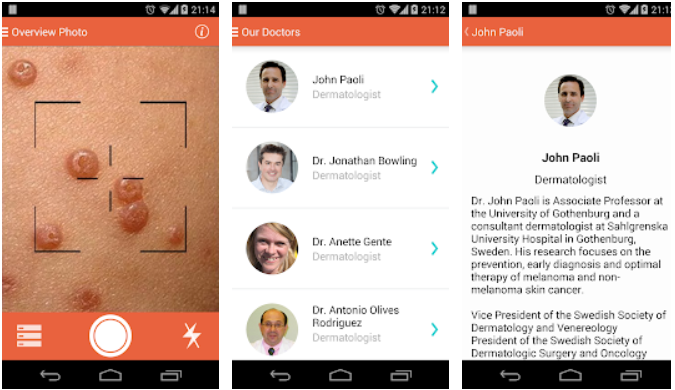
\includegraphics[height= 8cm, width=9cm]{backmatter/figures/IDoc24.PNG} 
 \caption{IDoc24}
 \end{figure}
 
 
\subsection{First Derm}
The team behind iDoc24 also developed and operated the First Derm platform, which is very similar to the iDoc24 app: it allows access to a dermatologist through a connected device.\\

Launched in 2014 as an iOS app, available in six languages, it diagnoses 14 types of skin conditions and above all provides mothers with an on-the-go skin care assessment tool as a first step around skin care concerns within their families, including infants and children.\\

Worries only send pictures of mosquito bites or rashes of their young children to a licensed dermatologist connected via the app anonymously, the pictures will be reviewed and real dermatologists answer your query within hours. 
(And they don't use Dermatology AI - which is not accurate.)
\begin{figure}[H]
 \centering 
 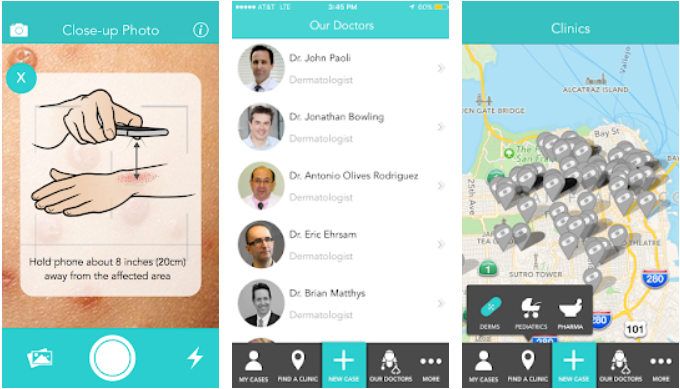
\includegraphics[height= 8cm, width=9cm]{backmatter/figures/FirstDerm1.PNG}
 \caption{First Derm}
 \end{figure}
 
\subsection{Cureskin (Acne, Pimples, Skin \& Hairfall Treatment: CureSkin)}
Cureskin is intended to help alleviate the situation. It can diagnose six types of common skin conditions - pimples, acne, scars, dark spots, pigmentation and dark circles.\\

The app's chatbot asks a few questions and poses artificial intelligence, based on the input. I recommend an eight-week skincare regimen.\\

CureSkin is a skin care app trusted by over 12 users for skin problems and hair loss. Once you place the order, your customized CureSkin set will be delivered.\\
Safe and tested products for pregnant women and new mothers.
 \subsubsection{Pros:}
 \begin{itemize}
     \item Safe and Confidential - All your data remains 100\% safe and confidential.\\
     \item With 100\% accuracy.\\
 \end{itemize}
\subsubsection{Cons:}
\begin{itemize}
     \item Diagnosed only six types of common skin diseases.\\
\end{itemize}

\subsection{SkinVision -  Find Skin Cancer }
SkinVision is a regulated medical service that enables you to take charge of the health of your skin.
With a smartphone app at the core of its service, SkinVision expands your ability to self-examine your skin, diagnose just one disease and provide fast and accurate skin cancer detection, along with the most reliable personal advice on skin health and health path recommendation.
 \subsubsection{Pros:}
 \begin{itemize}
     \item With 95\% accuracy.\\
 \end{itemize}
\subsubsection{Cons:}
\begin{itemize}
     \item Only one disease diagnosed.\\
\end{itemize}
\begin{figure}[H]
 \centering 
 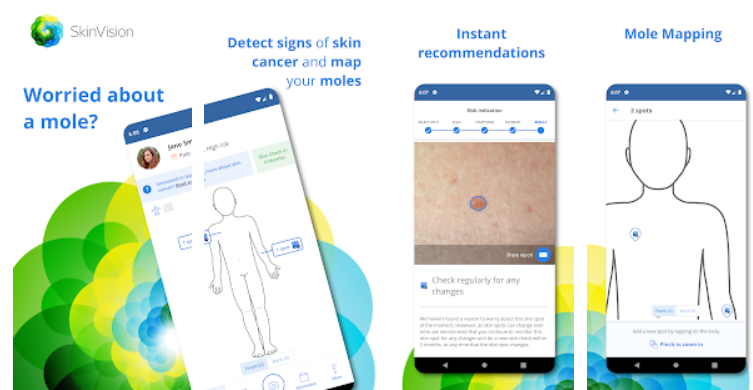
\includegraphics[height= 8cm, width=9cm]{backmatter/figures/SkinVision.PNG}
 \caption{SkinVision}
 \end{figure}
 
\subsection{Skin Diseases and Treatments}
This app covered most of the dermatology as it provided a resource for people diagnosed with new skin diseases. You can recognize the disease just by seeing it in a good descriptive picture of each disease separately, and gives skin care tips (by experts)
 \subsubsection{Pros:}
 \begin{itemize}
     \item Provides excellent and extensive satisfactory data.\\
 \end{itemize}
\subsubsection{Cons:}
\begin{itemize}
     \item Only 47 diseases diagnosed.\\
\end{itemize}

\begin{figure}[H]
 \centering 
 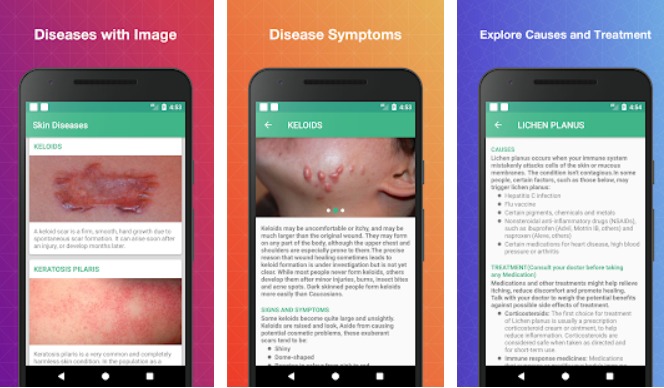
\includegraphics[height= 8cm, width=9cm]{backmatter/figures/SkinDandTreatment.PNG}
 \caption{Skin Diseases and Treatments}
 \end{figure}
 
\subsection{Aysa, your answer to common skin conditions}
Aysa is the easy-to-use app for getting personalized answers to your skin condition questions.\\

Aysa helps you check your skin symptoms and prepare for your practitioner visit.
Use the phone's camera to take a picture of your skin problem and Aysa will quickly find a match for your symptoms to provide personalized and helpful information about your symptoms Aysa is built on the resources of VisualDx, the award-winning clinical decision support program that has focused on equity in medicine for over 20 years. Its curated library of more than 120,000 medical images.\\

The workflow also allows you to select skin tone, ensuring the best possible information and images.
Aysa's knowledge and recommendations are based on the best available evidence required according to industry standard protocols, which are interpreted through expert opinion.
 \subsubsection{Pros:}
 \begin{itemize}
     \item Your privacy is protected with Apple's CoreML (Machine Learning).\\
     \item High accuracy.\\
 \end{itemize}
\subsubsection{Cons:}
\begin{itemize}
     \item Only 200 skin diseases were diagnosed.\\
\end{itemize}
\begin{figure}[H]
 \centering 
 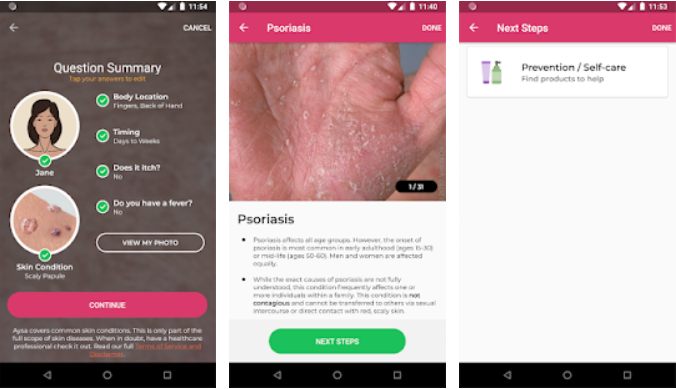
\includegraphics[height= 8cm, width=9cm]{backmatter/figures/Aysa.PNG}
 \caption{Aysa, your answer to common skin conditions}
 \end{figure}
\newpage
\section{Relationship between the Relevant Work and Our Own Work }
There have been a number of real applications running as we have previously reviewed, but they are limited to a small number of diseases and lack the precision to be independent.So a system aims to fix both problems, as we have a system that is able to diagnose more than \textbf{620 skin diseases} with better accuracy overall, plus the models can be updated without crashing the system as a whole.\\
Improving accuracy is detrimental to the application of disease diagnosis, and to achieve this, the models are divided into two layers.\\

\textbf{The first layer} is for classification which is simply to output which of the 23 general skin conditions the entry belongs to,\\
That is when \textbf{the second layer}  begins whose function is to determine exactly what type of disease is being introduced.\\\\
New technologies are being taken into consideration such as cloud computing which will enable us to have a large number of independent models running simultaneously with virtually no delay in response.\\\\
\textbf{Last but not least,} the drastic changes in mobile devices and networks over the past two years enable us to use high-resolution images to feed our AI models, moreover, the preprocessing phase will be used to increase the accuracy of the models.\\\\

\section{Summary }
Our project presents a proposed solution that depends on the presence of any mobile device connected to the Internet.\\
\textbf{The diagnostic process goes as follows:}\\
\textbf{First:} the patient asks for a new examination followed by two simple questions, such as the affected place on the body for example.\\
\textbf{Second,} he will be asked to provide an image of the area related to the diagnosis, and he may also be asked to cut out only that particular area for easier detection.\\
\textbf{Finally,} the patient is asked to confirm their input.\\

The result will be on top of the expected illnesses, as well as pictures of similar cases and information about the disease and what the patient can and cannot do to care for the affected area.\\
We also discussed in this chapter academic researchers and scientists
Existing papers that provide the same service, also show basic information, as we have explained the most important libraries, tools and software technologies used in our project.\\\\
\large \textbf{Finally, }we discuss the relationship between our intended project and related work process
Taking into account all the advantages and disadvantages to reach our goal by developing and improving this service by increasing the number of diseases that we diagnose and increasing the accuracy of the models.
